\documentclass[xcolor=dvipsnames]{beamer}


\usepackage[T1]{fontenc}
\usepackage[utf8]{inputenc}


\usepackage[french]{babel}
\usepackage{graphicx}%@@final
\usepackage{hyperref}
\usepackage{amsmath}
\usepackage{listings}
\usepackage{diagbox}
\usepackage{tikz}
\usetikzlibrary{shapes} 
\usepackage{xcolor}
\usepackage{url}
\usepackage{array}
 
 
\lstset{tabsize=2, numbers=left, numberstyle=\tiny, stepnumber=5, numbersep=5pt,breaklines=true,
    emph={int}, emphstyle=\color{red},
    emph={[2]int,for}, emphstyle={[2]\color{red}},
    emph={[3]int,for,printf}, emphstyle={[3]\color{blue}},
    morecomment=[s][\color{green}]{/*}{*/}
}
 
\newcolumntype{P}[1]{>{\centering\arraybackslash}p{#1}} 
 
 
\usetheme{Pittsburgh}
%\setbeamercovered{invisible}  
%\useinnertheme[shadow=true]{rounded}
%\useoutertheme{infolines}
\usecolortheme{dove}
\setbeamerfont{block title}{size={}}
\setbeamercolor{titlelike}{parent=structure,bg=white} 
\setbeamercolor{item}{fg=RedOrange}

\setbeamertemplate{footline}[frame number]
 
\hypersetup{%colorlinks,%
%citecolor=black,%
%filecolor=black,%
%linkcolor=black,%
urlcolor=red}
 
\author {Nicolas Paliod, Martin Chevalier}

\title{Estimation de variance \\ dans les enquêtes de l'Insee : le \textit{package} R gustave}
\institute{10ème Colloque francophone sur les sondages \\ Session Estimation de variance et Robustesse}

\AtBeginSection[]
 {
 \begin{frame}<beamer>
 \frametitle{Plan}
 \tableofcontents[sectionstyle = show/shaded,hideallsubsections]
 \setcounter{tocdepth}{1}
 \end{frame}
 }

\date{26 octobre 2018}

\begin{document}
\begin{frame}
\maketitle 
\begin{center}

\includegraphics[width=2cm]{logo.png}
\end{center}
\end{frame}

\section*{Introduction}

\begin{frame}{Pourquoi calculer la variance d'un indicateur ?}

\begin{itemize}
    \item L'estimation de variance est importante \textcolor{red}{pour le chargé d'études} :
    \begin{itemize}
        \vspace{0.1cm}
        \item Permet de disposer d'un intervalle de confiance
        \vspace{0.1cm}
        \item Permet de commenter la significativité des variations de l'indicateur
    \end{itemize}
    
    \vspace{0.2cm}
    \item L'estimation de variance permet de \textcolor{red}{mesurer la qualité des indicateurs produits}
    \begin{itemize}
        \vspace{0.1cm}
        \item Utilisée pour les rapports qualité transmis à Eurostat
        \vspace{0.1cm}
        \item Requise pour divers indicateurs dans différentes enquêtes par le nouveau règlement européen IESS (\textit{Integrated european social statistics}) en discussion
    \end{itemize}
    
    \vspace{0.2cm}
   
    \item L'estimation de variance est donc une opération qui gagne en importance \textcolor{red}{dans le processus de production d’une enquête}
\end{itemize}

\end{frame}

\begin{frame}{Les sources d'erreurs dans une enquête}
Chaque maillon de la chaîne de production d'une enquête peut être source d'erreur :

\begin{itemize}
    \item Base de sondage
    \item Plan de sondage
    \item Taille de l'échantillon
    \item Estimateur retenu
    \item Spécification des questions
    \item Réponse aux questions
    \item Non-réponse
    \item Chaînes de traitement des données
\end{itemize}

Ces erreurs recouvrent biais et incertitude.

\end{frame}

\begin{frame}{Les parties de la chaîne de production prises en compte par les estimations de variance à l'Insee}
    
\begin{itemize}
    \item Eléments liés au plan de sondage :
    \begin{itemize}
        \vspace{0.2 cm}
        \item Algorithmes de tirage
        \vspace{0.2 cm}
        \item Degrés de tirage
        \vspace{0.2 cm}
        \item Bases de sondage multiples
    \end{itemize}
    \vspace{0.5 cm}
    \item Eléments liés aux méthodes d'estimation
    \begin{itemize}
        \vspace{0.2 cm}
        \item Correction de la non-réponse
        \vspace{0.2 cm}
        \item Calage sur marges
    \end{itemize}
\end{itemize}
    
\end{frame}

\begin{frame}{Des solutions existantes mais imparfaites (1/2)}
\begin{itemize}
    \item \textcolor{red}{macro SAS \%calker} : sondage aléatoire simple stratifié, correction de la non-réponse par repondération ou par imputation au sein des strates de tirage \\ => pas adapté à des groupes de réponse homogènes
    
    \vspace{0.5 cm}
    
    \item \textcolor{red}{macro SAS \%calker\_grh} : sondage aléatoire simple stratifié, correction de la non-réponse par repondération au sein de groupes de réponse homogènes quelconques \\ => pas adapté à des plans de sondage complexes
    
\end{itemize}
\end{frame}

\begin{frame}{Des solutions existantes mais imparfaites (2/2)}
\begin{itemize}

    \item \textcolor{red}{macro SAS \%everest} : sondage aléatoire simple stratifié, correction de la non-réponse par imputation au sein des strates de tirage ou par repondération au sein de groupes de réponse homogènes quelconques, calage sur marges \\ => pas adapté à des plans de sondage complexes
    
    \vspace{0.5 cm}
    \item \textcolor{red}{macro SAS \%Poulpe} : estimateurs de variance s'appuyant sur les probabilités d'inclusion simple, modélisation générique du plan de sondage et des phases de redressement, modules de linéarisation intégrés \\ => pas adapté à l'utilisation en production par un chargé d'études
    
\end{itemize}
\end{frame}

\section{Objectifs du package}

\begin{frame}{Trois grands objectifs}

\textit{package} R \textcolor{red}{G}ustave : a \textcolor{red}{U}ser-oriented \textcolor{red}{S}tatistical \textcolor{red}{T}oolkit for \textcolor{red}{A}nalytical \textcolor{red}{V}ariance \textcolor{red}{E}stimation

\vspace{0.5 cm}

3 objectifs axés autour de :
\vspace{0.3 cm}

\begin{itemize}
    \item user
    \vspace{0.3 cm}
    \item toolkit
    \vspace{0.3 cm}
    \item analytical variance estimation
\end{itemize}

\end{frame}

\begin{frame}{Un \textit{package} de calcul de variance analytique}
\begin{itemize}
    \item \textcolor{red}{Systématiser le calcul de variance} en s'abstrayant des éléments communs à tous les calculs de variance, à toutes les enquêtes
    \vspace{0.5cm}
    \item Le \textit{package} permet de \textcolor{red}{prendre en compte simplement} :
    \vspace{0.2 cm}
    \begin{itemize}
        \item \textcolor{red}{le calage sur marges} (fonction \textit{res\_cal})
        \vspace{0.2 cm}
        \item \textcolor{red}{l'estimation sur un domaine} (arguments \textit{by}, \textit{where})
        \vspace{0.2 cm}
        \item \textcolor{red}{la linéarisation} (fonctions de linéarisation \textit{mean}, \textit{ratio}, \textit{diff\_of\_ratio},  \textit{ratio\_of\_ratio})
    \end{itemize}
\end{itemize}
\end{frame}

\begin{frame}{Un \textit{package} orienté utilisateur}

\begin{itemize}
    
    \item \textcolor{red}{Simplifier le calcul de variance} en limitant le travail du méthodologue au codage de la fonction d'estimation de variance analytique adapté à l'enquête
    
    \vspace{0.5 cm}
    
    \item \textcolor{red}{Standardiser la mise en forme} des fonctions de calcul de variance, avec des fonctions déjà présentes dans le package, pour permettre au chargé d'études de récupérer une fonction d'estimation de variance simple d'utilisation
    
\end{itemize}
    
\end{frame}

\begin{frame}{Une boîte à outils}

Un \textit{package} qui permet au méthodologue :

\vspace{0.5 cm}

\begin{itemize}
    
    \item d'intégrer dans la fonction d'estimation de variance n'importe quelle étape de l'enquête pourvu qu'il existe un calcul analytique qui puisse être codé
    \vspace{0.3 cm}
    \item de disposer de fonctions déjà codées

\end{itemize}
    
\end{frame}

\begin{frame}{Faire interagir les différents acteurs du processus de production}

Le \textit{package} permet à chaque acteur du processus de production de limiter son travail à son champ d'action :

\begin{itemize}
    \vspace{0.3 cm}
    \item \textcolor{red}{le chargé d'études} pour la production d'estimations de variance d'indicateurs
    \vspace{0.3 cm}
    \item \textcolor{red}{le méthodologue} pour la production de la fonction d'estimation de variance adaptée à l'enquête
    \vspace{0.3 cm}
    \item \textcolor{red}{le développeur} pour améliorer l'ergonomie des fonctions de variance produites par le package, pour intégrer de nouvelles fonctionnalités
\end{itemize}

\end{frame}

\section{Fonctionnement du package}

\begin{frame}{Le \textit{wrapper} de variance}

Parmi les objectifs :

\begin{itemize}
    \vspace{0.2 cm}
    \item intégrer des fonctionnalités communes pour toutes les enquêtes comme l'estimation sur un domaine
    \vspace{0.2 cm}
    \item avoir une mise en forme standard des fonctions de variance pour simplifier leur utilisation
\end{itemize}

\vspace{0.5 cm}
\textcolor{red}{Solution} mise en \oe uvre : \textcolor{red}{le \textit{wrapper} de variance}

\begin{itemize}
    \vspace{0.2 cm}
    \item define\_variance\_wrapper() : fonction générique qui prend en charge des opérations systématiques (statistiques de linéarisation, domaines), appelle la fonction d'estimation de variance et affiche les résultats
\end{itemize}
    
\end{frame}

\begin{frame}{Des fonctions de variance déjà codées dans le \textit{package}}
    
Le \textit{package} contient \textcolor{red}{un certain nombre de fonctions} utiles dans différentes enquêtes :
\vspace{0.2 cm}
\begin{itemize}
    \item des fonctions d'estimation de variance analytique
    \begin{itemize}
        \item Variance de Sen-Yates-Grundy
        \vspace{0.1 cm}
        \item Variance de Deville-Tillé (Deville, Tillé, 2005)
    \end{itemize}
    \vspace{0.2 cm}
    \item des statistiques de linéarisation (\textit{mean}, \textit{ratio}, \textit{diff\_of\_ratio},  \textit{ratio\_of\_ratio})
\vspace{0.2 cm}
    \item une fonction \textit{res\_cal} pour prendre en compte le calage
\end{itemize}

\end{frame}

\begin{frame}{L'utilisation du package gustave à l'Insee}

\begin{itemize}
    \item Utilisé pour l'estimation de variance des enquêtes ménages périodiques : 
    \vspace{0.1 cm}
    \begin{itemize}
        \item Enquête emploi en continu (EEC)
        \item Dispositif Statistique sur les revenus et les conditions de vie (SRCV)
        \item Cadre de vie et sécurité (CVS)
        \item Loyers et charges
    \end{itemize}
    \vspace{0.2 cm}
    \item \textcolor{red}{Exemple : Enquête emploi en continu}
    \vspace{0.1 cm}
    \begin{itemize}
        \item panel de logements initialisé en 2009, tirage équilibré
        \item correction de la non-réponse par calage en une étape
        \item indicateurs standards : ratios (taux de chômage, etc.) ventilés par domaine
    \end{itemize}

\end{itemize}

\vspace{0.2 cm}
\footnotesize{\textcolor{red}{Nota bene} Les estimateurs ponctuels figurant sur les diapositives suivantes ne coïncident en général pas avec la diffusion officielle (champs de calcul différents, pas de désaisonnalisation, etc.)}

\end{frame}

\begin{frame}{Exemple de calcul de variance à l'Insee (1/3)}
    
\begin{itemize}
    \item \textcolor{red}{Première phase :} préparation des données pour qu'elles contiennent toutes les variables ensuite utilisées par la fonction de variance codée en deuxième phase
    \vspace{0.5 cm} 
    \item \textcolor{red}{Deuxième phase :} codage de la fonction de variance
\end{itemize}

\begin{center}
    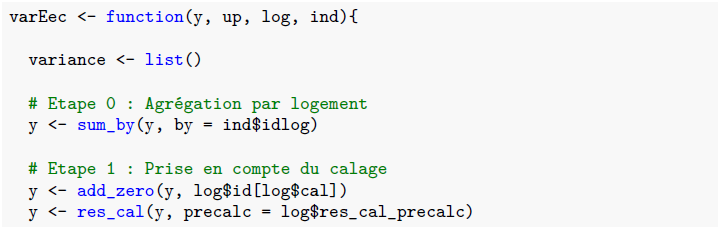
\includegraphics[width = 10 cm]{EEC_1.png}
\end{center}    

\end{frame}

\begin{frame}{Exemple de calcul de variance à l'Insee (2/3)}
    
\begin{center}
    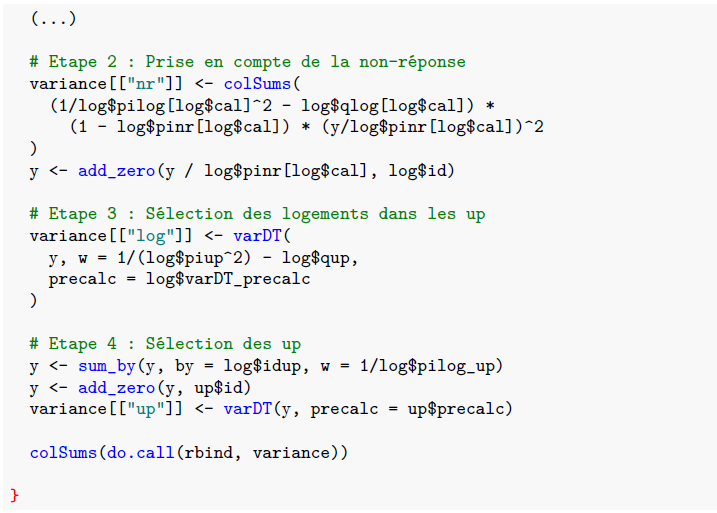
\includegraphics[width = 10 cm]{EEC_2.png}
\end{center}

\end{frame}

\begin{frame}{Exemple de calcul d'estimation de variance à l'Insee (3/3)}

\begin{itemize}
    \item \textcolor{red}{Troisième phase :} à partir de la fonction de variance et de l'information auxiliaire nécessaire, la fonction define\_variance\_wrapper() crée un \textit{wrapper} de variance simple d’utilisation
\end{itemize}

\begin{center}
    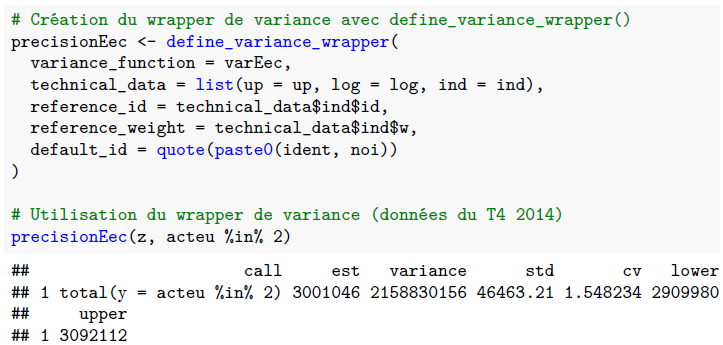
\includegraphics[width = 10 cm]{EEC_3.png}
\end{center}

\end{frame}

\begin{frame}{Contraintes de diffusion}

\begin{itemize}
    \item \textcolor{red}{Remarque pour la diffusion de la fonction de variance produite :} \\ \vspace{0.2 cm} Le \textit{wrapper} de variance est une fonction complètement autonome : \textcolor{red}{toute l'information auxiliaire spécifiée au paramètre technical\_data est intégrée dans la fonction} (il s'agit d'une \textit{closure})
\end{itemize}

\end{frame}

\begin{frame}{La fonction qvar()}

\begin{itemize}
    \item La fonction qvar() : \og \textcolor{red}{une fonction prête-à-estimer} \fg \ pour des plans de sondage simples et des redressements standards
    
    \vspace{0.5 cm}
    
    \item La fonction qvar() \textcolor{red}{combine les autres fonctions} du package gustave
    
    \vspace{0.5 cm}
    
    \item La fonction qvar() s'applique dans un \textcolor{red}{cadre similaire à la macro SAS \%everest} :
    \vspace{0.1 cm}
    \begin{itemize}
        \item sondage aléatoire simple stratifié
        \vspace{0.1 cm}
        \item correction de la non-réponse par repondération dans des groupes de réponse homogènes
        \vspace{0.1 cm}
        \item calage sur marges
    \end{itemize}
\end{itemize}
    
\end{frame}

\begin{frame}{Un \textit{package} pensé pour être extensible (1/3)}

La fonction define\_variance\_wrapper() accepte \textcolor{red}{n'importe quelle fonction de variance en entrée}: 
\vspace{0.2cm}
\begin{itemize}
    \item autant d'information auxiliaire que nécessaire
    \vspace{0.1 cm}
    \item utilisation des fonctions d'autres \textit{packages} pour coder la fonction de variance (utiliser require() dans la fonction de variance)
\end{itemize}

\vspace{0.4 cm}
Large éventail de méthodologies couvert à ce jour : 
\vspace{0.2cm}
\begin{itemize}
    \item échantillons tirés dans l'échantillon-maître Octopusse (formule spécifique dérivée de la formule de Sen-Yates-Grundy (Chauvet, 2011 et Gros, Moussallam, 2015))
    \vspace{0.1cm}
    \item degrés multiples (CVS)
    \vspace{0.1cm}
    \item partage des poids complexes (SRCV)
\end{itemize}

\end{frame}

\begin{frame}{Un \textit{package} pensé pour être extensible (2/3)}

La fonction de variance peut exporter, en plus des variances estimées, des \textcolor{red}{résultats intermédiaires} de l'estimation de variance.
    
\vspace{0.4 cm}

Cette fonctionnalité facilite la création de \textcolor{red}{surcouches} à partir des \textit{wrappers} de variance produits par le \textit{package} gustave.

\vspace{0.4 cm}

\textcolor{red}{Exemple} : Dans l'EEC, l'estimation de variance pour des indicateurs faisant intervenir plusieurs trimestres (évolution d'un trimestre à l'autre, moyennes annuelles, etc.) s'appuie sur la récupération des résultats intermédiaires des \textit{wrappers} de variance de chaque trimestre concerné (estimation des covariances trimestrielles).

\end{frame}

\begin{frame}{Un \textit{package} pensé pour être extensible (3/3)}

Il est également possible de définir de nouvelles fonctions pour estimer la précision de \textcolor{red}{statistiques complexes} grâce à la fonction define\_statistic\_wrapper() :

\begin{center}
    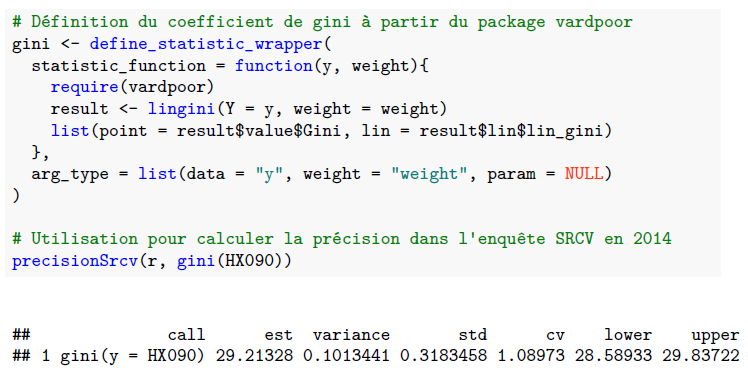
\includegraphics[width = 10 cm]{gini.png}
\end{center}    

\end{frame}


\section{Principe et outils de développement}

\begin{frame}{Diffusion sur le Cran, tests unitaires et intégration en continu}

\begin{itemize}
    \item \textit{package} disponible sur le \underline{\href{https://cran.r-project.org/web/packages/gustave/index.html}{Cran}}, dernière version : août 2018
    \vspace{0.5 cm}
    \item Le développement sous la forme de \textit{packages} favorise également le développement de \textcolor{red}{tests unitaires}
    \vspace{0.2 cm}
    \begin{itemize}
        \item à chaque fonctionnalité du \textit{package} est associé un \textcolor{red}{test} qui vérifie son bon fonctionnement
        \vspace{0.2 cm}
        \item gustave comporte plus de \textcolor{red}{180 tests unitaires}
        \vspace{0.2 cm}
        \item à chaque nouvelle version du \textit{package}, des tests sont automatiquement réalisés : \textcolor{red}{intégration en continu}
    \end{itemize}
\end{itemize}
    
\end{frame}

\begin{frame}{Suivi de versions}

Les évolutions du \textit{package} sont \textcolor{red}{suivies en version} depuis l'été 2017 :

\begin{itemize}
    \vspace{0.1 cm}
    \item \textcolor{red}{code source librement accessible} sur plusieurs plateformes de développement, notamment \underline{\href{https://github.com/martinchevalier/gustave}{github.com}}

    \vspace{0.1 cm}

    \item \textcolor{red}{conservation de toutes les versions} (plus de 300 \textit{commits} à ce jour) avec leurs métadonnées : une description est associée à chaque ensemble cohérent de modifications

    \vspace{0.1 cm}

    \item \textcolor{red}{travail collaboratif facilité}, y compris de façon concomittante : création de branches pour des développements particuliers, gestion des conflits

    \vspace{0.1 cm}

    \item possibilité pour des utilisateurs externes de \textcolor{red}{proposer efficacement des modifications} (remontée de \textit{bugs}, demandes spécifiques, \textit{pull requests})
\end{itemize}
    
\end{frame}

\section*{Conclusion}

\begin{frame}{Conclusion}

Le Département des méthodes statistiques de l'Insee a mis en place un \textit{package} R pour \textcolor{red}{systématiser l'estimation de variance} :
\vspace{0.1 cm}
\begin{itemize}
    \item une solution qui permet à chaque participant de la chaîne de production de se préoccuper uniquement de la partie qu'il a en charge
    \vspace{0.1 cm}
    \item des fonctions d'estimation de variance simples d'utilisation
    \vspace{0.1 cm}
    \item un \textit{package} documenté
\end{itemize}

\vspace{0.5 cm}

Un \textit{package} \textcolor{red}{déjà utilisé pour les enquêtes ménages de l'Insee} :
\begin{itemize}
    \vspace{0.1 cm}
    \item pour produire les estimations de variance jointes aux rapports qualité
    \vspace{0.1 cm}
    \item pour vérifier le respect des objectifs de précision prévus par le règlement IESS
\end{itemize}

\end{frame}

\end{document}
